\documentclass[a4paper,12pt]{article}
\usepackage[T2A]{fontenc}
\usepackage[utf8]{inputenc}
\usepackage[top=2cm, bottom=2cm, right=2cm, left=2cm]{geometry}
\usepackage[russian]{babel}
\usepackage{pscyr}
\usepackage{indentfirst}
\usepackage{graphicx}
\usepackage{epstopdf}
\usepackage{amstext}
\usepackage{amssymb}
\usepackage{amsmath}
\usepackage{cmap}
\usepackage{enumitem}
\usepackage{subcaption}
\pdfminorversion=6
%\input{environment}
%\linespread{1.3}
\tolerance=1000 
\hfuzz=0pt
\parindent=1.27cm
\captionsetup[table]{name = Таблица, labelsep = endash, justification=raggedright, singlelinecheck=false}
\captionsetup[figure]{name = Рисунок, labelsep = endash}
%\sloppy
%\RequirePackage{caption}
%\DeclareCaptionLabelSeparator{defffis}{ -- }
%\captionsetup{justification=centering,labelsep=defffis}

\graphicspath{{images/}{models/}}

\begin{document}
	\newcommand\tline[2]{$\underset{\text{#1}}{\text{\underline{\hspace{#2}}}}$}
	\begin{titlepage}
		\centering
		{\fontsize{12pt}{5cm}\selectfont \bfseries Министерство образования и науки Российской Федерации} \\ \vspace{0.5cm}
		{\fontsize{7pt}{5cm}\selectfont ФЕДЕРАЛЬНОЕ ГОСУДАРСТВЕННОЕ АВТОНОМНОЕ ОБРАЗОВАТЕЛЬНОЕ УЧРЕЖДЕНИЕ ВЫСШЕГО ПРОФЕССИОНАЛЬНОГО ОБРАЗОВАНИЯ} \\ 
		\vspace{1cm}
		{\fontsize{12pt}{5cm}\selectfont \bfseries САНКТ-ПЕТЕРБУРГСКИЙ УНИВЕРСИТЕТ ИНФОРМАЦИОННЫХ ТЕХНОЛОГИЙ, МЕХАНИКИ И ОПТИКИ} \\ \vspace{1.5cm}

		{\fontsize{14pt}{5cm}\selectfont Кафедра \hspace{1cm} \underline{Систем Управления и Информатики}  \hspace{1cm} Группа \underline{Р3340}} \\ 
		\vspace{2cm}

		{\fontsize{20pt}{5cm}\selectfont \bfseries Лабораторная работа №8} \\
		{\fontsize{20pt}{5cm}\selectfont \bfseries “Экспериментальное построение областей устойчивости линейной системы на плоскости двух параметров”} \\
		{\fontsize{14pt}{5cm}\selectfont Вариант - 5} \\
		\vspace{1.5cm}

		\flushleft

		{Выполнил \hspace{2cm} \tline{(фамилия, и.о.)}{9cm} (подпись)} \\
		\vspace{2cm}

		{Проверил \hspace{2cm} \tline{(фамилия, и.о.)}{9cm} (подпись)} \\
		\vspace{5cm}

		"\underline{\hspace{0.7cm}}"\hspace{0.2cm}\underline{\hspace{2cm}}\hspace{0.2cm}20\underline{\hspace{0.7cm}}г. \hspace{2cm} Санкт-Петербург, \hspace{2cm} 20\underline{\hspace{0.7cm}}г. \\ \vspace{1cm}

		Работа выполнена с оценкой \hspace{1cm} \underline{\hspace{8cm}} \\ 
		\vspace{1cm}
		Дата защиты "\underline{\hspace{0.7cm}}"\hspace{0.2cm}\underline{\hspace{2cm}}\hspace{0.2cm}20\underline{\hspace{0.7cm}}г.

	\end{titlepage}
	\paragraph{Цель работы.} Ознакомление с экспериментальными методами построения областей устойчивости линейных динамических систем и изучение влияния на устойчивость системы ее параметров.
	
	\paragraph {Исходные данные:} $g=0,~y(0)=1,~T_1=const=1.5,~T_2=var$\\
	\newpage
	\begin{center}
	\section{Моделирование системы}
	\end{center}
	Схема моделирования представлена на рисунке \ref{s_1}
	
	\begin{figure}[h]
		\renewcommand{\figurename}{Рисунок}
		\centering
		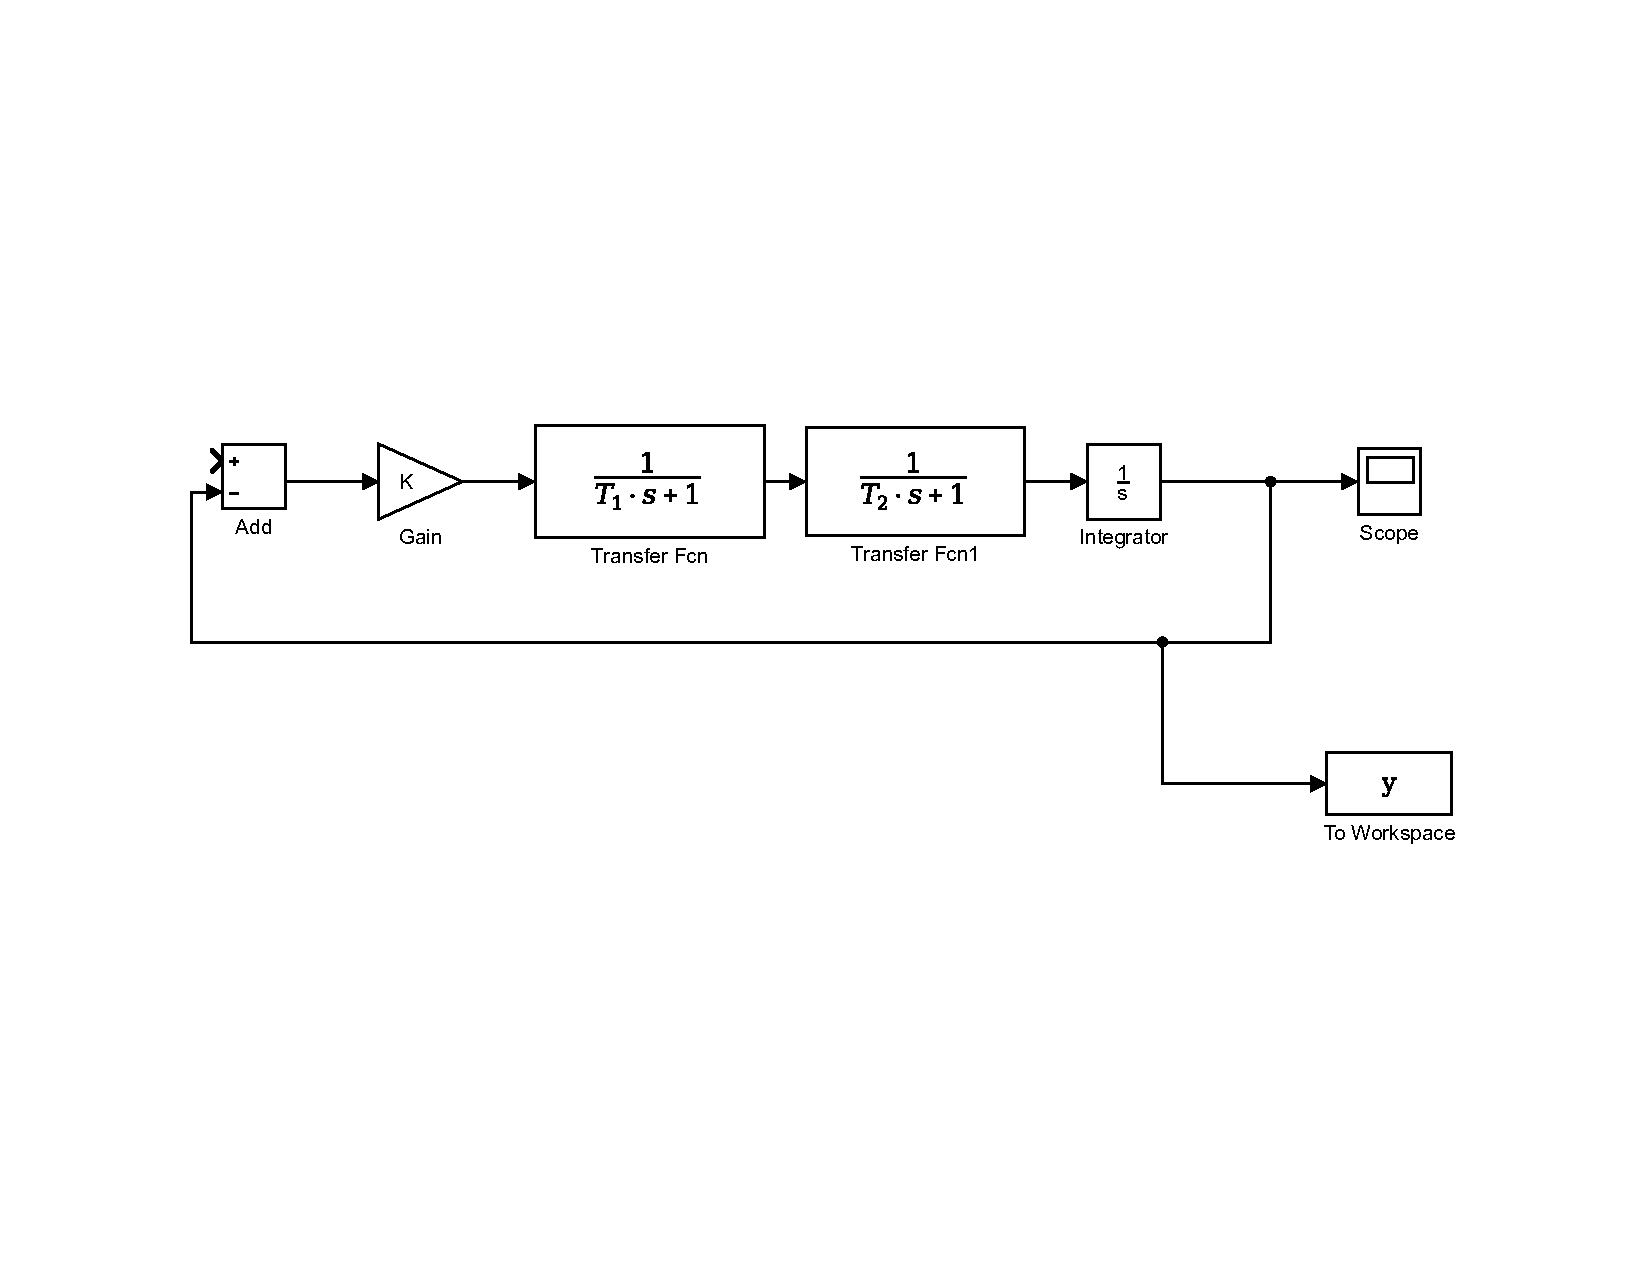
\includegraphics[width=6in]{Lab8MOD.pdf}
		\caption{Схема моделирования}
		\label{s_1}
	\end{figure}
	
	При $T_2=0.1$ и $K=5$ система устойчива, при $K=10.6$ система находится на колебательной границе, а при $K=15$ неустойчива. Все эти положения представлены на рисунке \ref{s_21} \ref{s_22} и \ref{s_23} соответственно.
	\begin{figure}[h!]
		\centering
			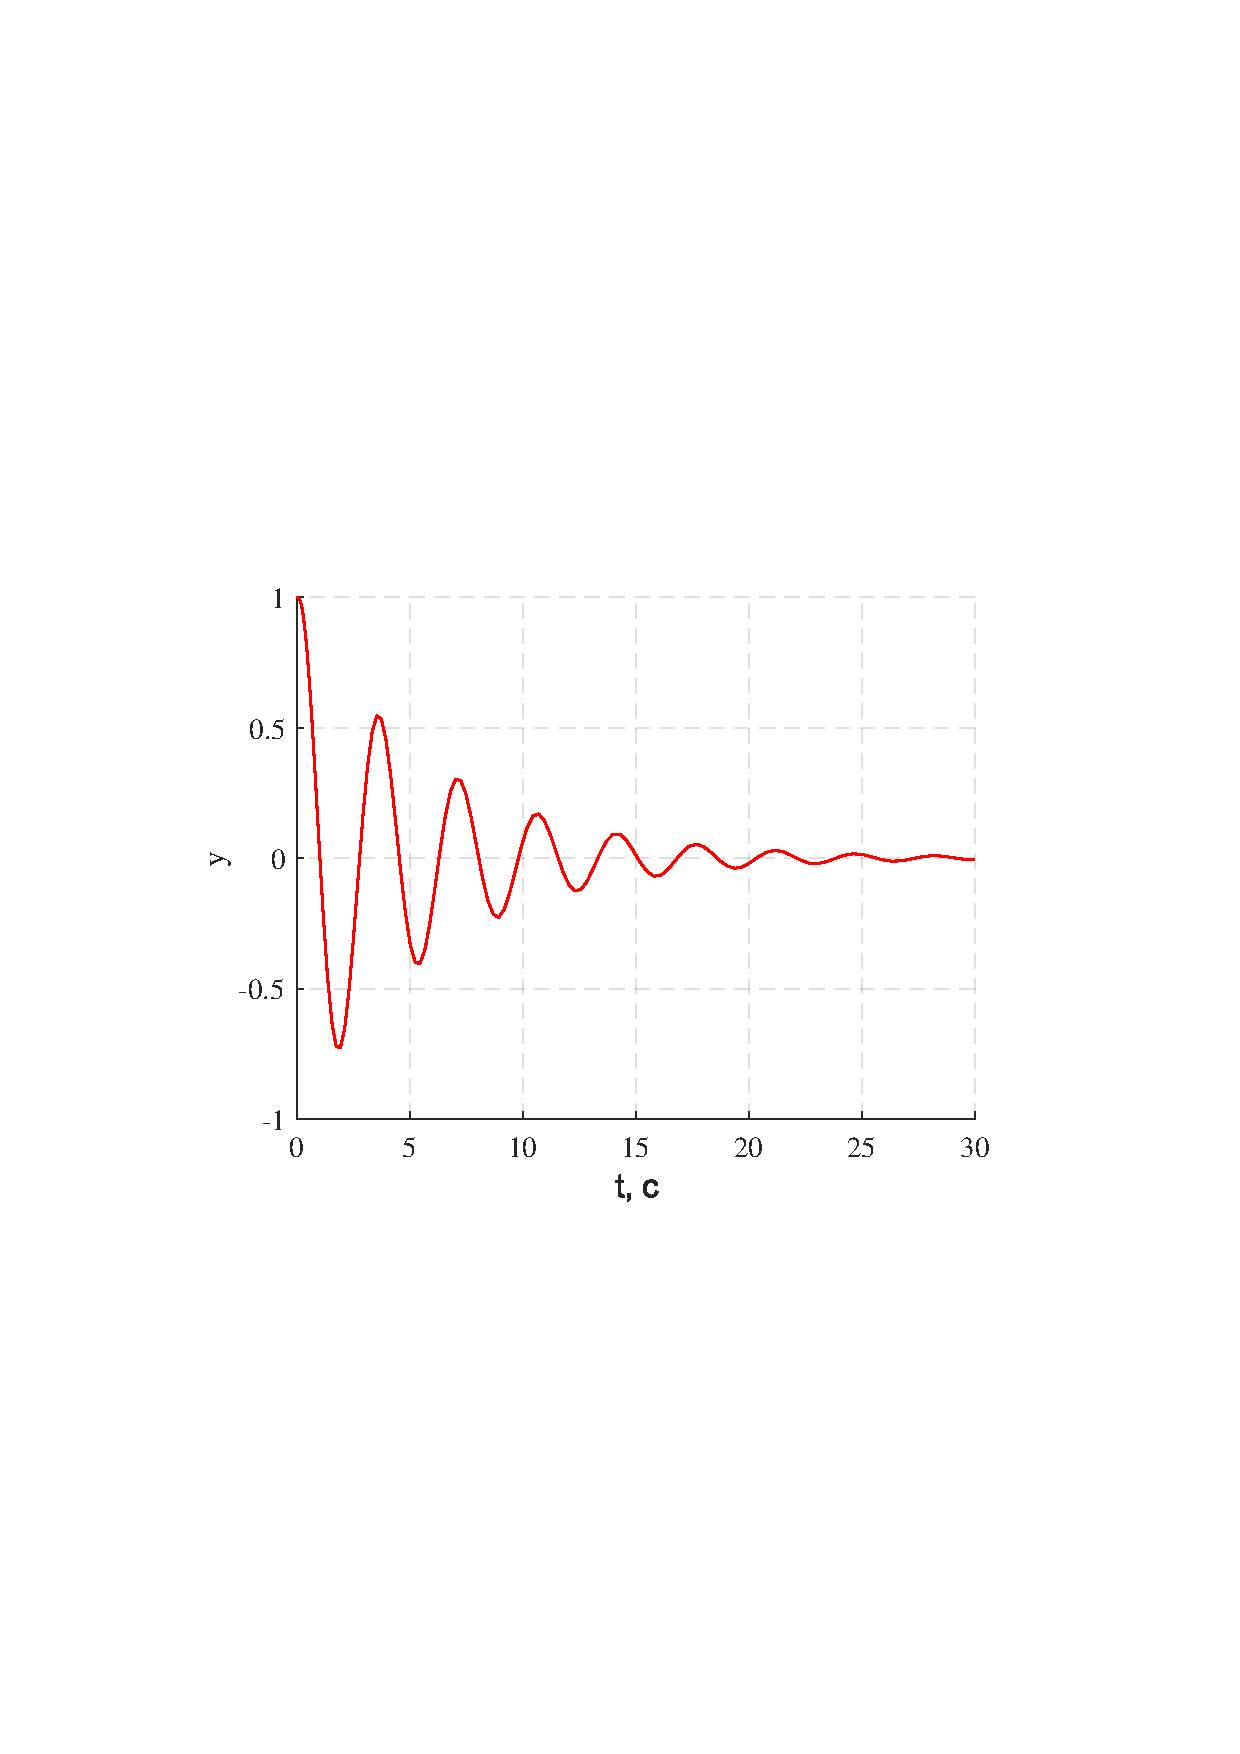
\includegraphics[width=6in]{UstoichivayaMOD.pdf}
			\caption{Устойчивая система}
			\label{s_21}
		\end{figure}
	\newpage			
				\begin{figure}[h!]
					\centering
					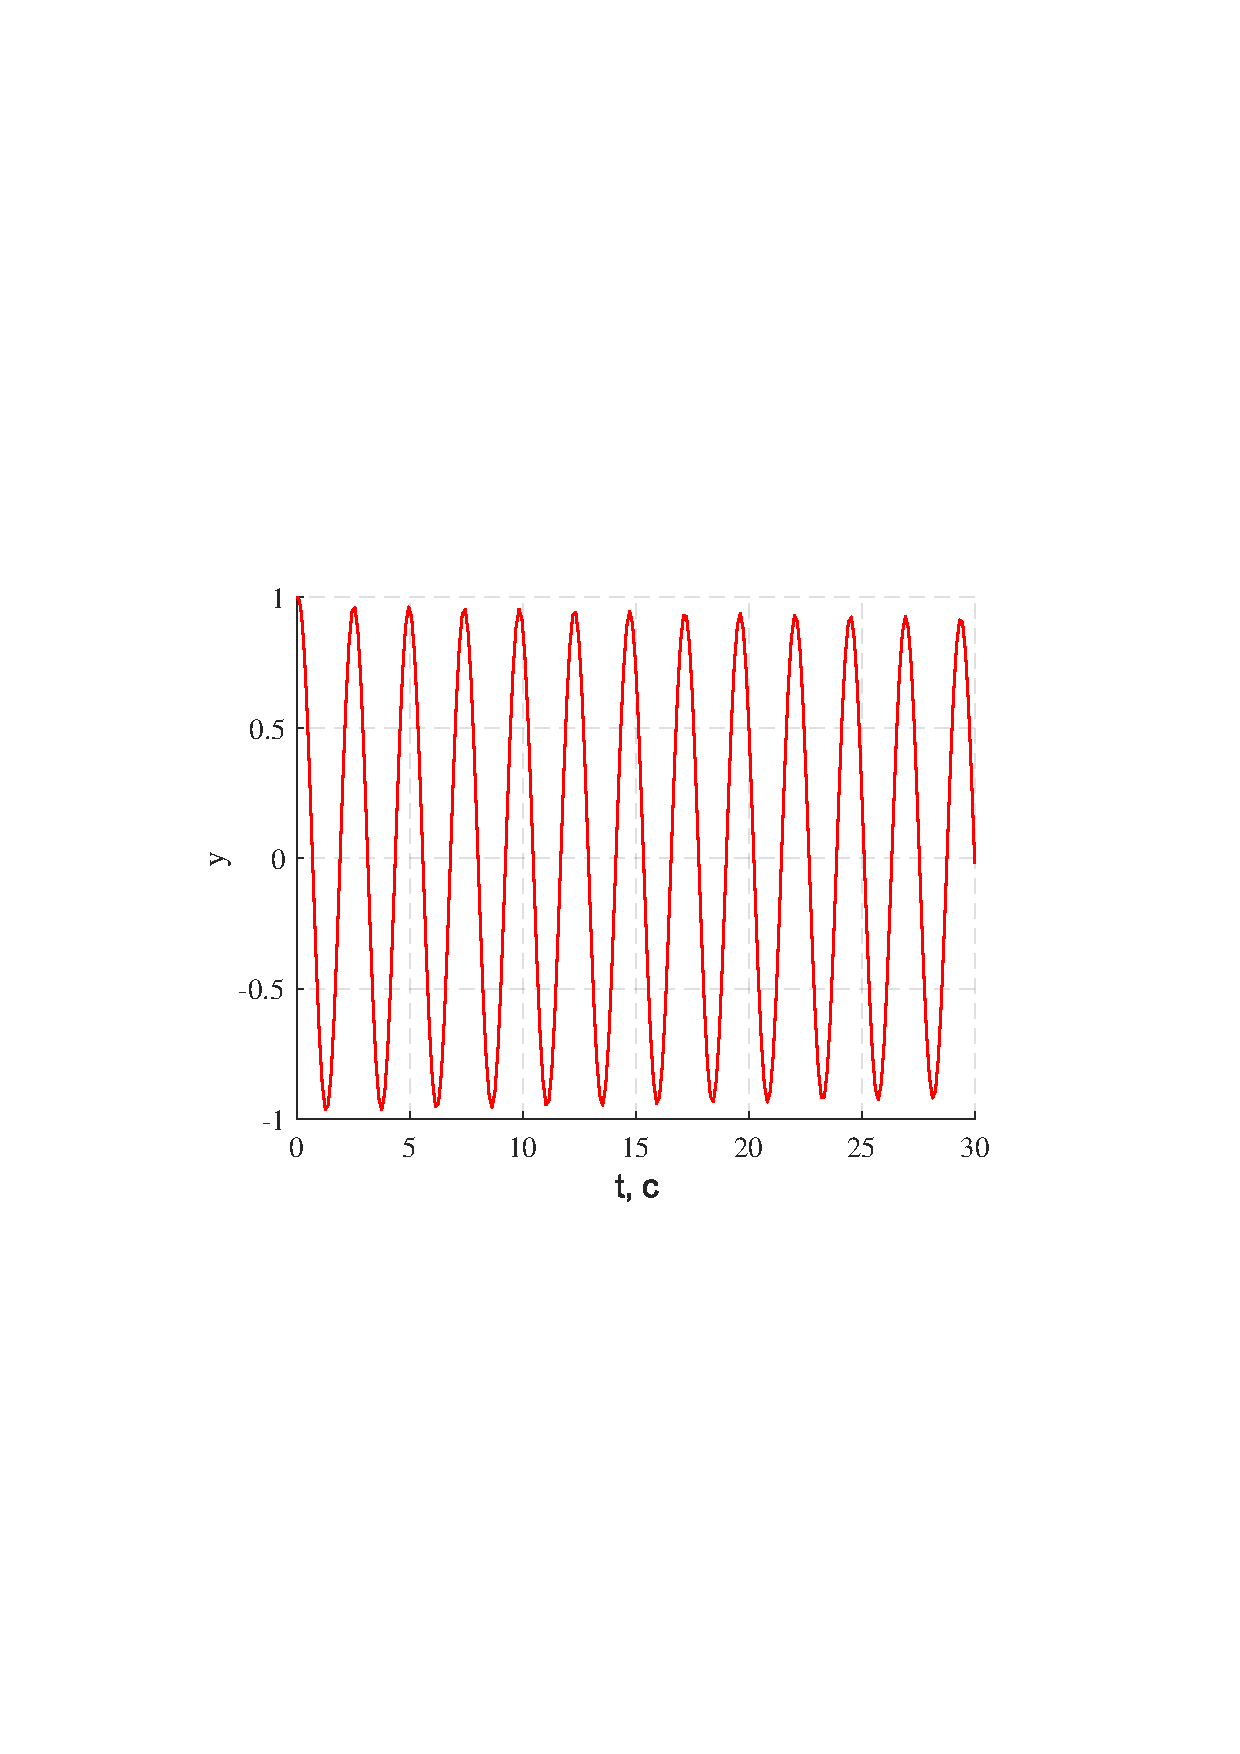
\includegraphics[width=6in]{KolebMOD.pdf}
					\caption{Система на колебательной границе устойчивости}
					\label{s_22}
				\end{figure}
						
		\begin{figure}[h!]
			\centering
			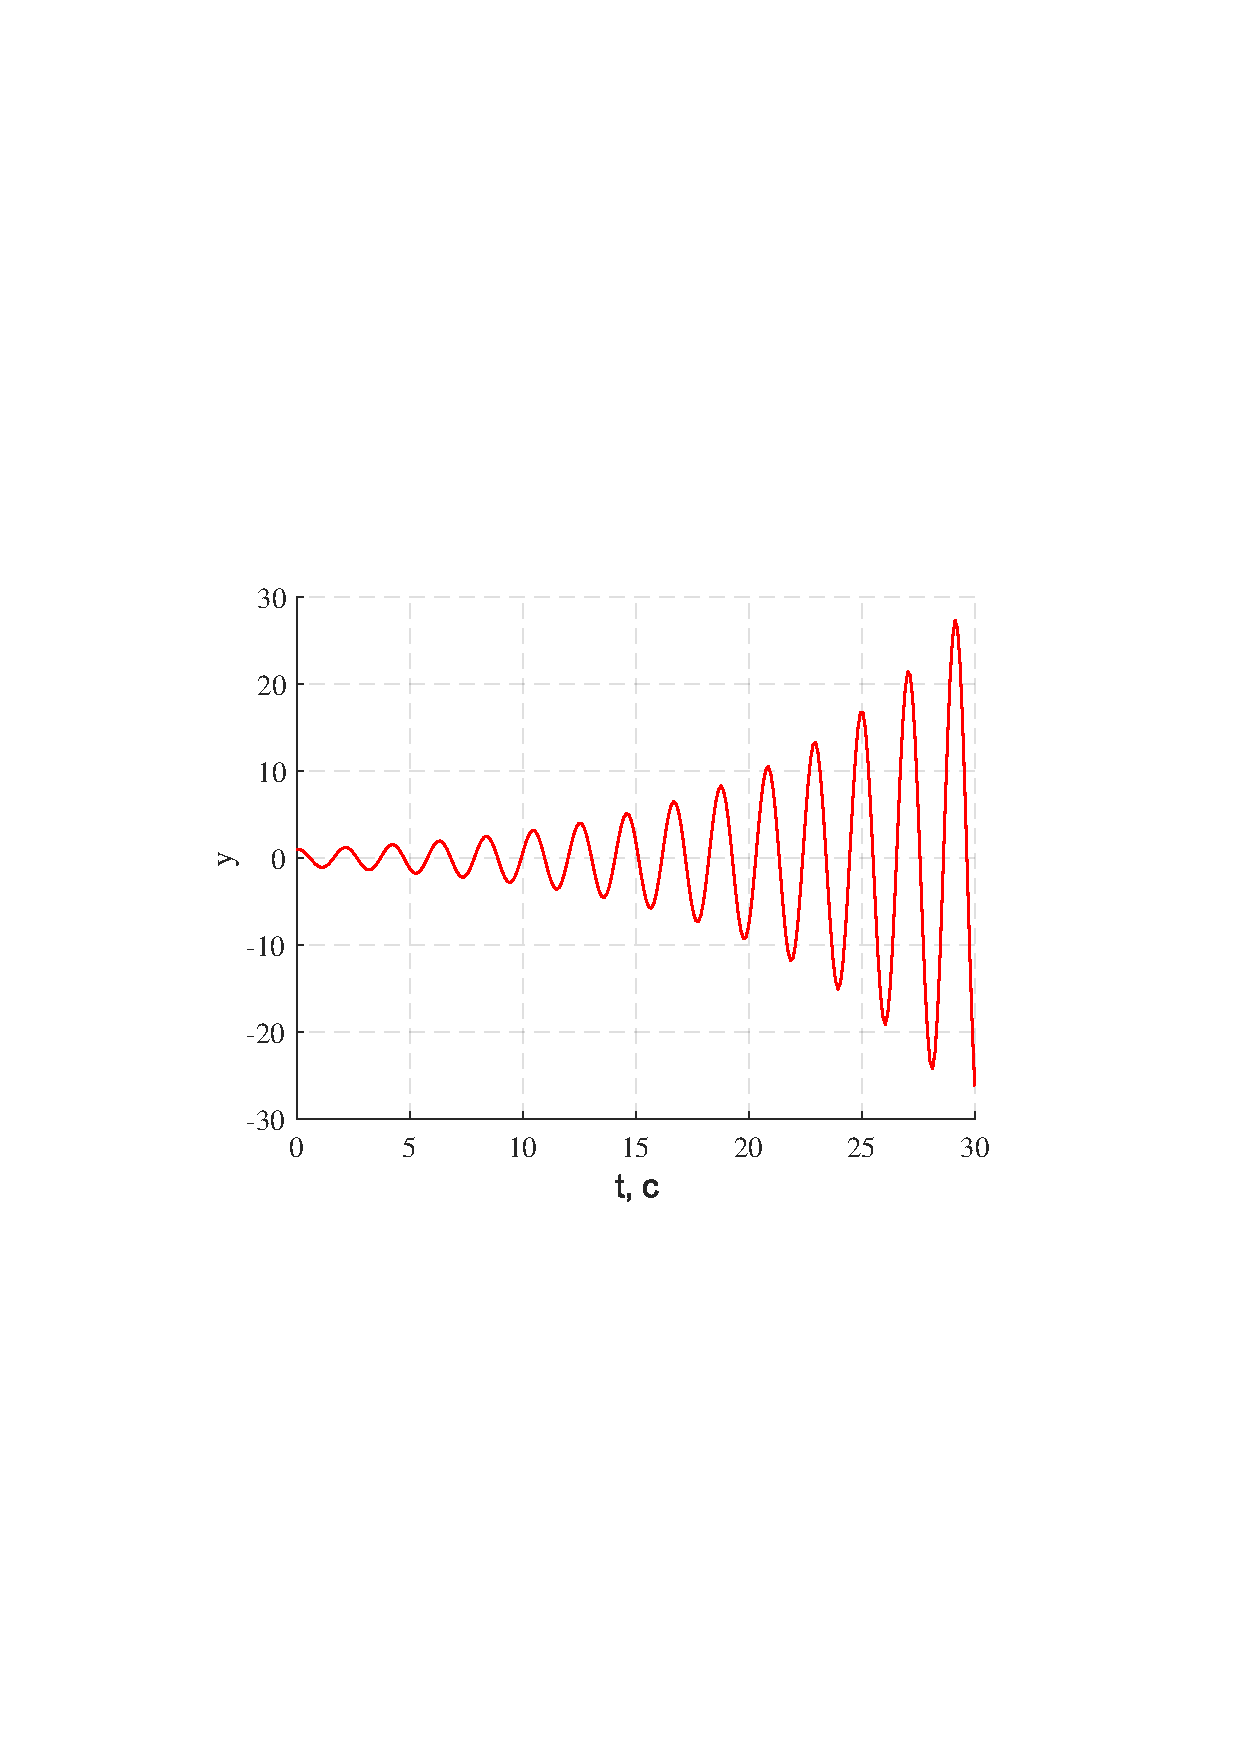
\includegraphics[width=6in]{NeustMOD.pdf}
			\caption{Неустойчивая система}
			\label{s_23}
		\end{figure}			





	\newpage
	\paragraph{} Будем изменять значение $T_2$ и искать значение $K$ при котором система находится на границе. Значения представлены в таблице \ref{t_1}, а получившаяся граница устойчивости - на рисунке \ref{s_3}
	\begin{table}[h]
		\caption{Данные моделирования}
		\renewcommand{\arraystretch}{2} 
		\renewcommand{\tabcolsep}{0.5cm}
		\begin{center}
			\begin{tabular}{|c|c|c|c|c|c|c|c|c|c|c|}
				\hline
				$T_2$, с & 0.1 & 0.5 & 1 & 1.5 & 2 & 2.5 & 3 & 3.5 & 4 & 4.5 \\ \hline
				$K$ & 10.6 & 2.7 & 1.7 & 1.35 & 1.2 & 1.1 & 1 & 0.95 & 0.9 & 0.85 \\ \hline
			\end{tabular}
		\end{center}
		\label{t_1}
	\end{table}
 
	\begin{figure}[h!]
		\renewcommand{\figurename}{Рисунок}
		\centering
		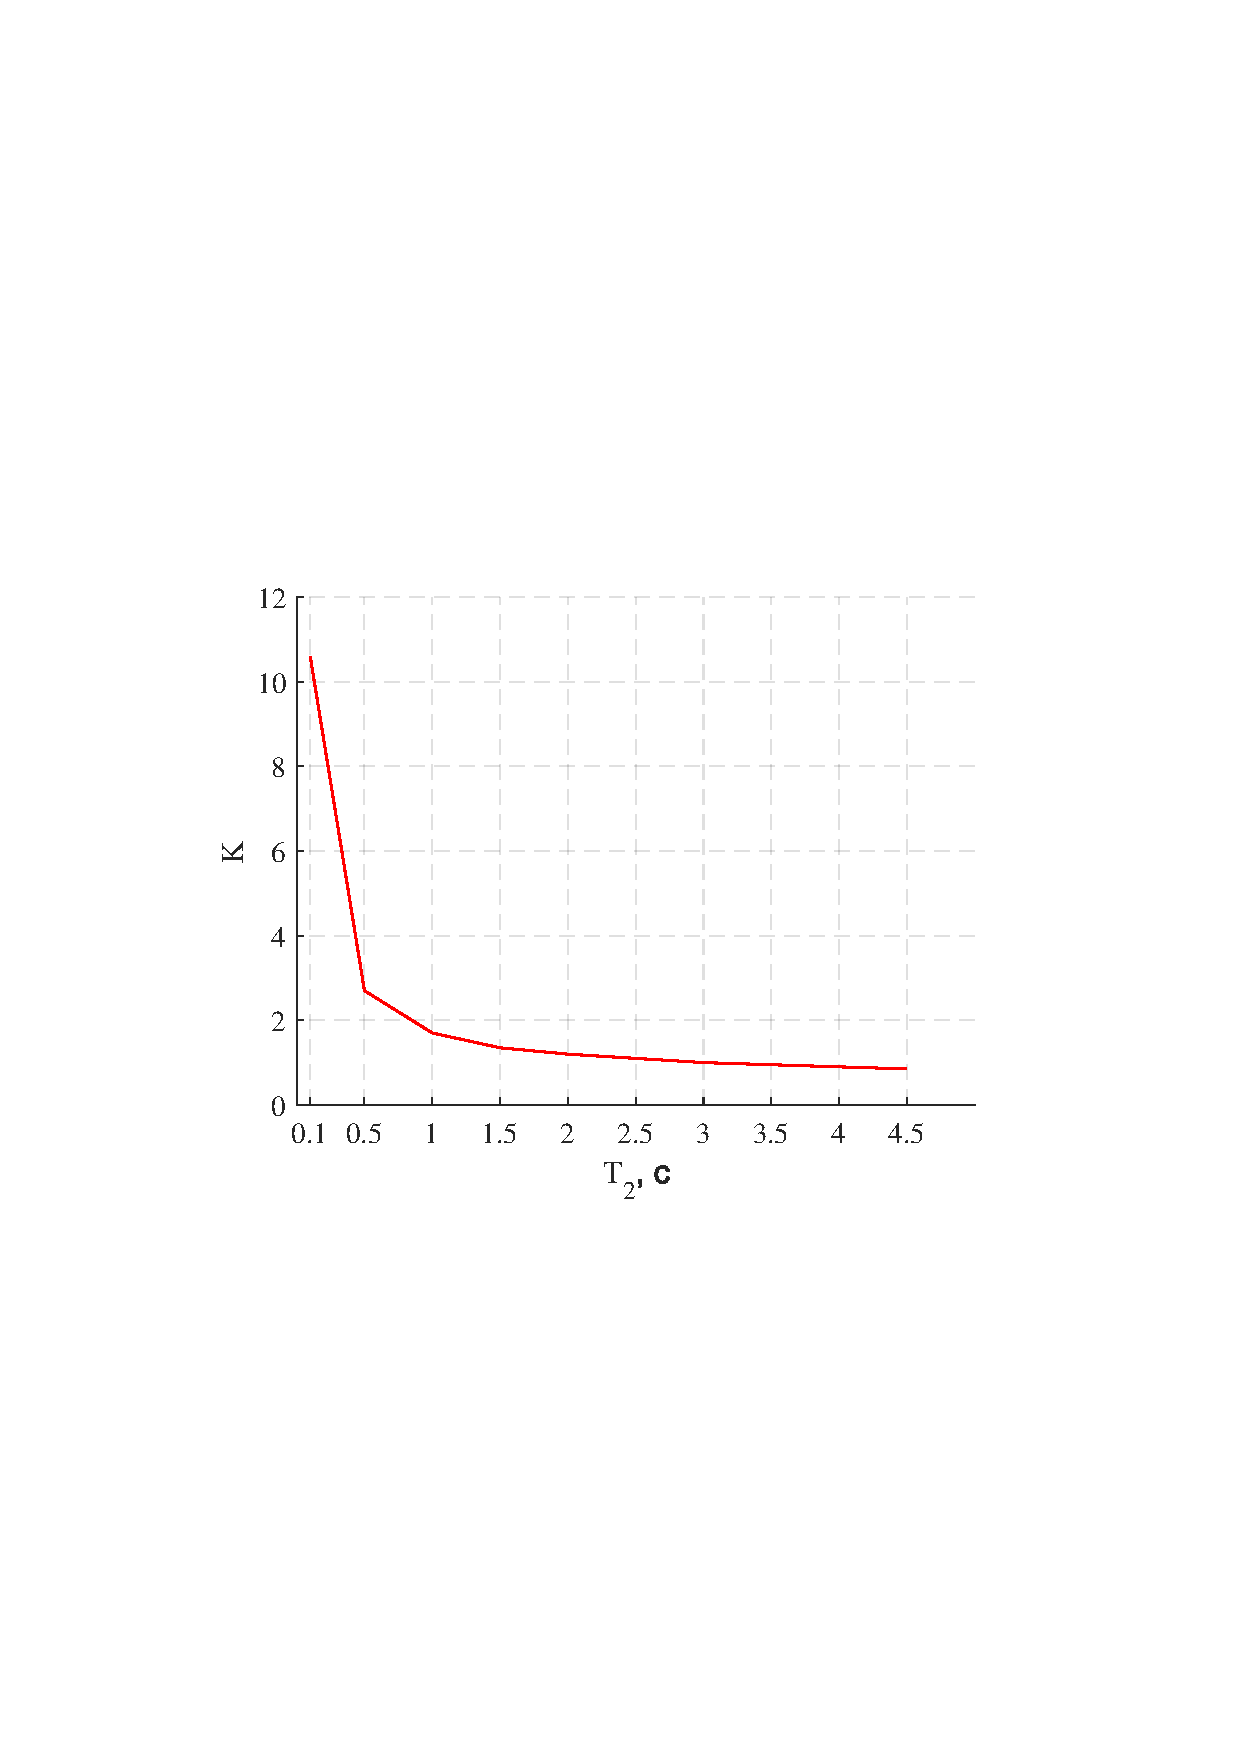
\includegraphics[width=6in]{GranitsaMOD.pdf}
		\caption{Граница устойчивости}
		\label{s_3}
	\end{figure}


	\clearpage
	
	\begin{center}
	\section{Теоретический расчет границы устойчивости с использованием критерия Гурвица}
	\end{center}
	\noindent
	
	\noindent Рассмотрим характеристический многочлен системы:\\
	\begin{gather}
	T_1T_2s^3+(T_1+T_2)s^2+s+K
	\end{gather}
	\par
	\noindent Составим матрицу Гурвица:\\
	\begin{gather}
	 \left( \begin{matrix} 
	T_1+T_2 & K & 0 \\ 
	T_1T_2 & 1 & 0 \\ 
	0 & T_1+T_2 & K \\ 
	\end{matrix} \right) 
	\end{gather}
	\\
	Для колебательной границы устойчивости должно выполняться равенство $K=\displaystyle\frac{T_1+T_2}{T_1T_2}$\\
	
	\noindent Рассчитаем значения $K$ при полученных ранее $T_2$. Результаты представлены в таблице \ref{t_2}, получившаяся граница устойчивости представлена на рисунке \ref{s_4}
	 \begin{table}[h]
	 	\caption{Расчетные данные}
	 	\renewcommand{\arraystretch}{2} 
	 	\renewcommand{\tabcolsep}{0.4cm}
	 	\begin{center}
	 		\begin{tabular}{|c|c|c|c|c|c|c|c|c|c|c|}
	 			\hline
	 			$T_2$, с & 0.1 & 0.5 & 1 & 1.5 & 2 & 2.5 & 3 & 3.5 & 4 & 4.5 \\ \hline
	 			$K$ & 10.67 & 2.67 & 1.67 & 1.34 & 1.17 & 1.07 & 1 & 0.95 & 0.92 & 0.89 \\ \hline
	 		\end{tabular}
	 	\end{center}
	 	\label{t_2}
	 \end{table}
	 
	 \begin{figure}[h]
	 	\renewcommand{\figurename}{Рисунок}
	 	\centering
	 	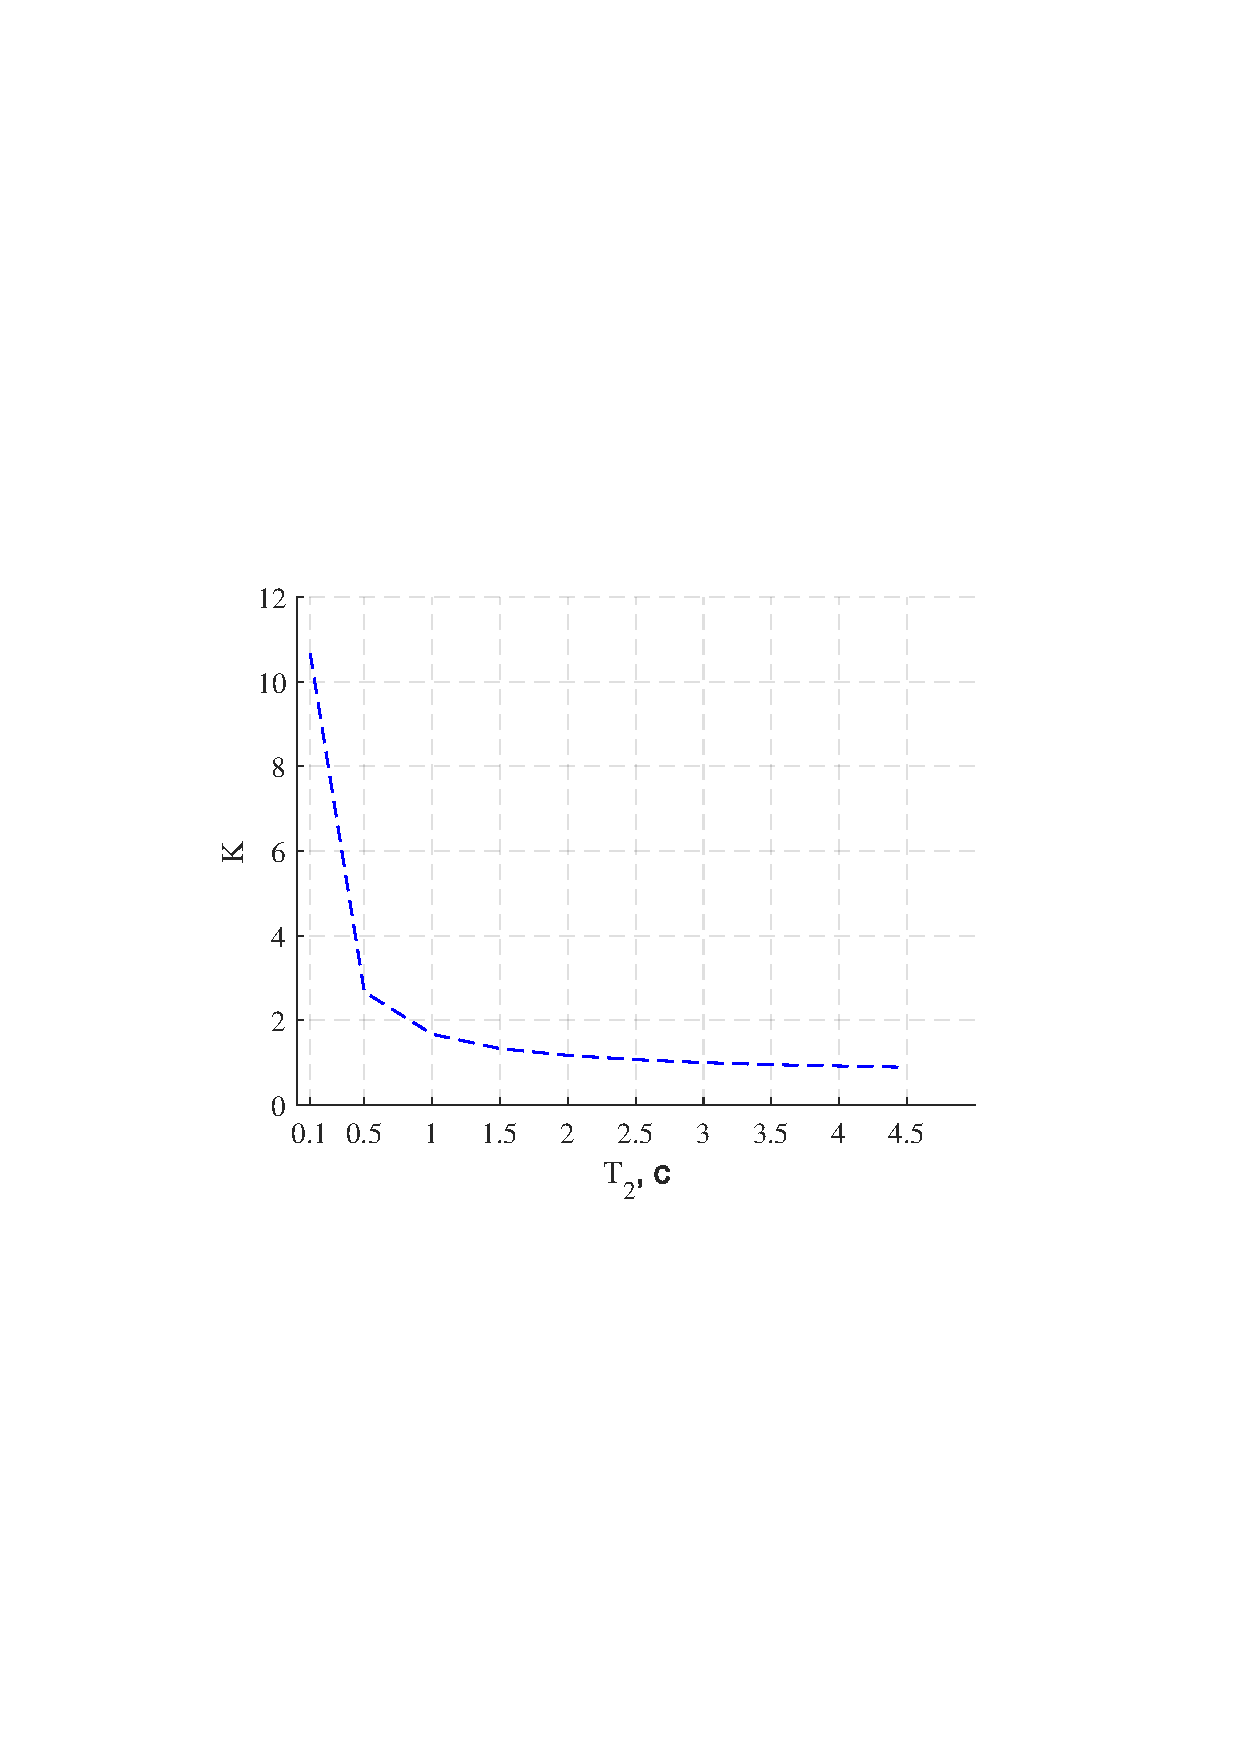
\includegraphics[width=6in]{RaschetMOD.pdf}
	 	\caption{Граница устойчивости}
	 	\label{s_4}
	 \end{figure}
 
 
 	\clearpage
 		\begin{center}
 	 \section{Выводы}
 		\end{center}
 	В данной работе была построена область устойчивости системы с помощью моделирования и аналитически: параметр $T$ оставался неизменным и для каждого $T_2$ находилось значение $K$, при котором система будет на границе.  
 	\par Также был произведен теоретический расчет границы устойчивости с помощью критерия Гурвица, результат которого совпал с результатом моделирования. 
	
	
	
	
\end{document}